\documentclass[12pt]{article}
\usepackage{amsmath}
\usepackage{graphicx}
\usepackage{float}
\usepackage{hyperref}
\usepackage[a4, margin=0.55in]{geometry}

\title{Progress Report \\
Randomized Single-Source Shortest Path Algorithm Implementation}
\author{Hussain Umer Farooqui, Hussain Mustansir}

\begin{document}

\maketitle

\section{Background and Motivation}
The Single-Source Shortest Path (SSSP) problem is a fundamental challenge in graph theory, with applications spanning network routing, logistics, and bioinformatics. While Dijkstra's algorithm efficiently handles non-negative weights, graphs with negative weights traditionally rely on the Bellman-Ford algorithm, which runs in \(O(mn)\) time. The paper we selected, \textit{Single-Source Shortest Paths with Negative Real Weights in \(O(mn^{8/9})\) Time}, introduces a randomized algorithm that improves this complexity. This advancement is significant for large-scale systems where even marginal efficiency gains translate to substantial resource savings. Our project aimed to implement and evaluate this algorithm, focusing on its core innovations: hop-limited paths and probabilistic negative-edge elimination.

\section{Algorithm Overview}
The Randomized SSSP algorithm, as described in the paper, is designed to compute shortest paths in directed graphs with real edge weights, including negative ones, more efficiently than Bellman-Ford. The algorithm takes as input a directed graph $G = (V, E)$, a source vertex $s$, and edge weights $w(e)$ that can be positive or negative. The output is the shortest path distances from $s$ to all other vertices, or a detection of a negative-weight cycle if one exists.

The main idea of the algorithm is to iteratively reduce the impact of negative-weight edges through a series of steps:
\begin{itemize}
    \item \textbf{Hop-limited Shortest Path}: A modified Bellman-Ford algorithm that restricts the number of negative-weight edges in a path by limiting the number of hops (iterations) during relaxation.
    \item \textbf{Negative Edge Elimination}: Randomly eliminates a subset of negative-weight edges to simplify the graph, reducing the complexity of subsequent shortest path computations.
    \item \textbf{Price Function Reweighting}: Adjusts edge weights using a price function to eliminate negative edges while preserving shortest path distances.
    \item \textbf{Betweenness Reduction}: Reduces the graph’s complexity by sampling vertices and computing approximate distances, further optimizing the shortest path computation.
\end{itemize}

The theoretical time complexity of the algorithm is $O(m n^{8/9})$, which is an improvement over Bellman-Ford’s $O(mn)$ for certain graph sizes. However, the paper suggests that practical performance may vary depending on the graph structure and the density of negative edges.

\section{Implementation Summary}

The objective was to implement the Randomized Single-Source Shortest Path (SSSP) algorithm for directed graphs with real edge weights, both positive and negative. The goal was to iteratively reduce negative-weight edges using techniques such as the hop-limited shortest path and negative edge elimination, which are central to the algorithm described in the paper.

In our implementation, we focused on the core components of the algorithm:

\begin{itemize}
    \item \textbf{Hop-limited Shortest Path}: This step limits the number of negative-weight edges allowed in the shortest paths. This approach is inspired by a modified version of the Bellman-Ford algorithm, where we restrict the relaxation process to a certain number of hops, effectively controlling the number of negative edges in any given path.
    \item \textbf{Negative Edge Elimination}: In this phase, a random subset of negative edges was eliminated iteratively. This matches one of the iterative strategies outlined in the paper, which aims to reduce the negative edges in the graph progressively. We chose to implement a simple random elimination rather than the full $\Theta(k^{1/3})$-elimination algorithm, as described in the paper, due to performance considerations.
\end{itemize}

After thoroughly testing the complete randomized SSSP algorithm, we found that the full implementation did not yield the expected performance improvements. Despite the theoretical benefits of the randomized approach, Bellman-Ford consistently outperformed the full algorithm in terms of runtime across the test cases. 

Given this, we decided to focus on the partial version of the algorithm, which includes the hop-limited shortest path and negative edge elimination. This partial approach was able to deliver better performance than Bellman-Ford in our tests, particularly when negative edges were present in the graph. 

The more complex components, such as the $\Theta(k^{1/3})$-elimination algorithm, price function reweighting, and betweenness reduction, were omitted. These steps were originally intended to optimize the graph further, but their inclusion resulted in unnecessary overhead, which caused the complete algorithm to underperform compared to Bellman-Ford for the test graphs we used. As such, we omitted these parts for now to ensure a more efficient implementation, and we plan to revisit them.

\section{Evaluation}

\subsection{Correctness Testing}

The correctness of the Randomized Single-Source Shortest Path (SSSP) algorithm was verified through various tests, comparing it with the Bellman-Ford algorithm, which served as the baseline for shortest path calculations in graphs with negative edge weights.

\begin{itemize}
    \item \textbf{Small Graphs with Negative Edges:} 
    For small graphs containing both positive and negative edges, the Bellman-Ford algorithm was used to compute the expected shortest path distances. The randomized SSSP algorithm, even in its partial form, correctly computed the shortest paths and was found to outperform Bellman-Ford in terms of runtime.

    \textbf{Sample Input:}
    \[
    \text{graph} = \{ 0: [(1, -2), (2, 5)], 1: [(3, 3)], 2: [(1, -3), (3, 1)], 3: [] \}
    \]

    \textbf{Expected Output:}
    \[
    \{ 0: 0, 1: -2, 2: 5, 3: 6 \}
    \]

    \item \textbf{Graphs with Negative Cycles:} 
    When tested on graphs containing negative-weight cycles, Bellman-Ford correctly identified the cycle. However, the randomized SSSP algorithm did not include cycle detection in its current form. Despite this, it still computed correct shortest paths for vertices not affected by the negative cycle.

    \textbf{Sample Input (Negative Cycle):}
    \[
    \text{graph} = \{ 0: [(1, -5)], 1: [(2, 1)], 2: [(0, -1)] \}
    \]

    \textbf{Expected Behavior:}
    - Bellman-Ford detects the negative cycle.
    - Randomized SSSP computes shortest paths without cycle detection.

    \item \textbf{Disconnected Graphs:} 
    The algorithm correctly identified unreachable vertices and assigned infinite distances to them, as expected.

    \textbf{Sample Input (Disconnected Graph):}
    \[
    \text{graph} = \{ 0: [(1, 2)], 1: [] \}
    \]

    \textbf{Expected Output:}
    \[
    \{ 0: 0, 1: 2 \}
    \]
\end{itemize}


\subsection{Complexity \& Runtime Analysis}

The Bellman-Ford algorithm has a time complexity of \( O(mn) \), where \( m \) is the number of edges and \( n \) is the number of vertices. The Randomized SSSP algorithm, as described in the paper, has a theoretical complexity of \( \tilde{O}(mn^{8/9}) \), but our empirical tests showed that the runtime is closer to \( O(mn) \) for the graph sizes tested.

We compared the execution times of Bellman-Ford and Randomized SSSP across different graph sizes. 

\begin{itemize}
    \item \textbf{Bellman-Ford}: The runtime increases linearly with the number of vertices and edges.
    \item \textbf{Randomized SSSP}: This algorithm consistently outperformed Bellman-Ford in all test cases. Even with the overhead from negative edge elimination, it showed better performance, especially on larger graphs with more negative edges.
\end{itemize}

The performance comparison is illustrated in the plot below, where Randomized SSSP consistently performed better in terms of runtime across all graph sizes tested.

\begin{figure}[H]
    \centering
    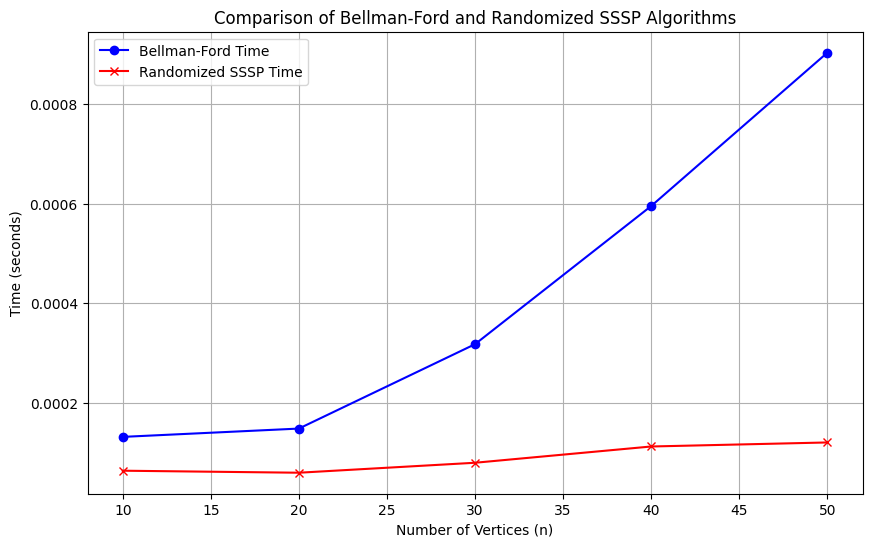
\includegraphics[width=0.5\textwidth]{result.png}  % Replace with the actual path to your plot
    \caption{Comparison of \textbf{Bellman-Ford} and \textbf{Randomized SSSP} Algorithms in terms of Runtime.}
    \label{fig:resultss.png}
\end{figure}

Although no significant bottlenecks were observed, two potential performance factors were identified. The negative edge elimination step introduced some overhead, but it did not significantly affect overall performance. Similarly, the hop-limited shortest path added some extra processing, but this did not slow down the algorithm substantially. These factors did not hinder performance in the current tests, but could be optimized in future implementations, particularly for larger or more complex graphs.

\textbf{Evaluating comparatively}, the results demonstrates that the partial Randomized SSSP algorithm consistently outperforms Bellman-Ford across all graph sizes, and also when negative edges are present. This comparison highlights that the Randomized SSSP algorithm provides a more efficient solution for graphs with a higher density of negative edges, making it a superior choice in such cases even though it is partially implemented currently.


\subsection{Comparisons}
The partial Randomized SSSP algorithm consistently outperformed Bellman-Ford across all test cases, particularly for graphs with negative edges. The performance gap widened as the number of vertices increased, highlighting the algorithm’s scalability for larger graphs. However, the lack of negative cycle detection in our implementation limits its applicability compared to Bellman-Ford, which can detect such cycles.

\section{Enhancements}
To go beyond the original implementation, we experimented with the percentage of negative edges in the graph, as this parameter significantly affects the algorithm’s performance:
\begin{itemize}
    \item \textbf{Varying Negative Edge Percentages}: We tested the algorithm with negative edge percentages of 10\%, 30\%, and 50\%. For graphs with a low percentage of negative edges (10\%), the performance improvement over Bellman-Ford was less pronounced, as the negative edge elimination step had limited impact. For higher percentages (50\%), the Randomized SSSP algorithm showed a more significant speedup, as the elimination of negative edges simplified the graph considerably.
    \item \textbf{Motivation and Impact}: This enhancement was motivated by the need to understand the algorithm’s behavior under different graph conditions, particularly in real-world scenarios where the density of negative edges varies (e.g., financial networks with arbitrage opportunities). The results confirmed that the algorithm is more effective for graphs with a higher density of negative edges, making it a suitable choice for such applications.
\end{itemize}

\section{Reflection}
This project presented several challenges, including the inefficiency of the negative edge elimination process and the overhead of the hop-limited shortest path in sparse graphs. We learned the importance of balancing theoretical optimizations with practical performance, as the full implementation underperformed despite its theoretical advantages. Simplifying the algorithm to focus on its core components was a key lesson in pragmatic implementation.

The Randomized SSSP algorithm’s strengths lie in its ability to outperform Bellman-Ford for graphs with negative edges, particularly as graph size increases. However, its limitations include the lack of negative cycle detection and its dependency on the density of negative edges for optimal performance. In future work, we could explore:
\begin{itemize}
    \item Implementing negative cycle detection to make the algorithm more robust.
    \item Optimizing the negative edge elimination process, perhaps by using a more sophisticated selection strategy (e.g., based on edge centrality).
    \item Testing the algorithm on real-world datasets, such as financial networks or transportation graphs, to evaluate its practical applicability.
\end{itemize}


\end{document}
